As power electronic converter systems become more complex, intelligent maintenance has emerged as a critical component for ensuring long-term operational reliability, safety, and economic performance. While the control layer governs real-time behavior, the maintenance layer focuses on assessing equipment health, anticipating failures, and optimizing lifecycle decisions. In this context, Deep Reinforcement Learning (DRL) offers unique advantages by enabling data-driven, adaptive, and scalable maintenance strategies that move beyond static rule- or threshold-based strategies. Fig.~\ref{fig:maintenance} presents a systematic flowchart of DRL maintenance activities in PECs. Generally, it consists of following three parts.

\begin{figure*}[t]
  \centering
  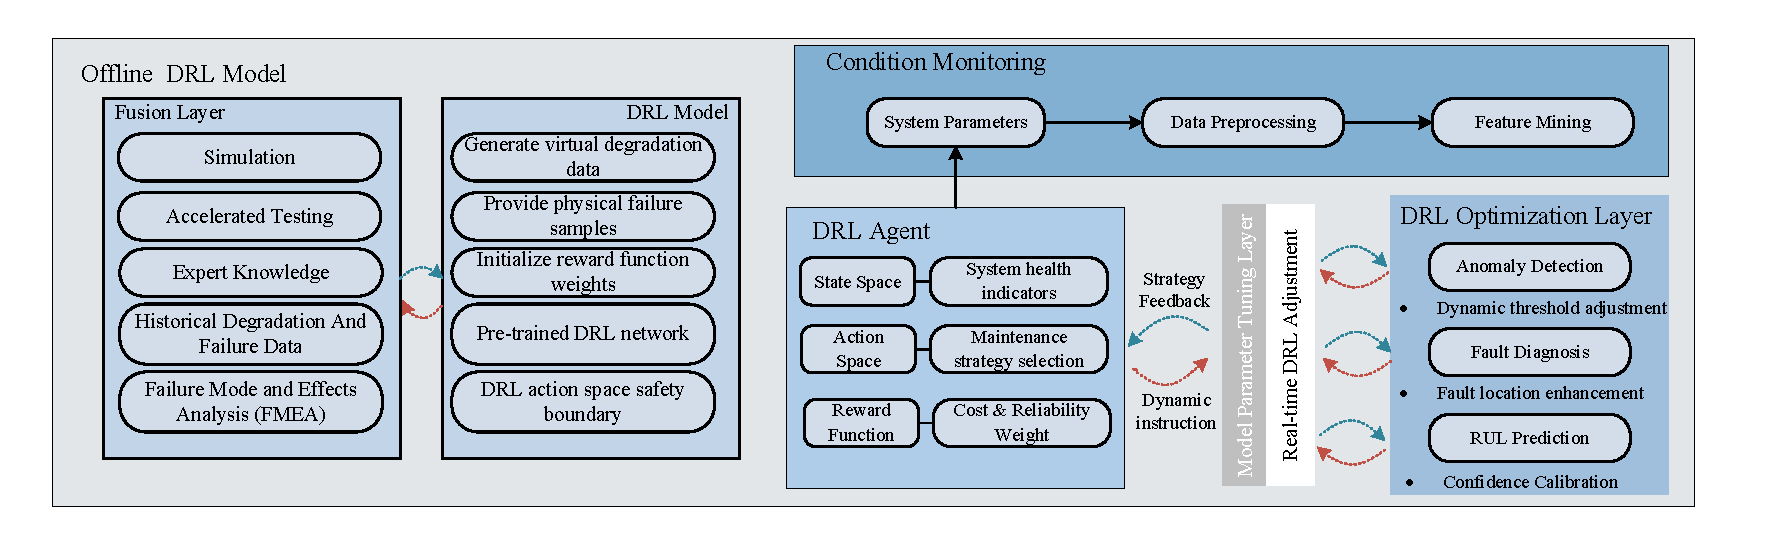
\includegraphics[width=\textwidth]{fig/maintenance.pdf}
  \caption{Flowchart of DRL maintenance in power electronic converter systems.}
  \label{fig:maintenance}
\end{figure*}


The application of DRL in converter maintenance can be structured into three interrelated domains:
\begin{enumerate}
  \item \textbf{Condition Monitoring}, which aims to continuously track system health through sensor data and latent state representations;
  \item \textbf{Anomaly Detection and Fault Diagnosis}, which identifies deviations from normal operation and localizes fault sources;
  \item \textbf{Remaining Useful Life (RUL) Prediction}, which estimates future degradation trajectories to support predictive or prescriptive maintenance planning.
\end{enumerate}

In the following subsections, we review recent advances in DRL-driven techniques for each of these tasks, highlighting their methodological innovations, application scenarios, and implementation challenges within converter-based energy systems.

\subsection{Condition Monitoring}
\label{Condition_Monitoring}
In the context of modern power electronic converter systems, condition monitoring serves as a foundational layer for intelligent maintenance by enabling continuous assessment of system health through real-time data acquisition and pattern recognition. As converters operate under increasingly dynamic and uncertain environments—often coupled with nonlinear interactions and varying load profiles—traditional monitoring approaches relying on threshold-based detection or fixed statistical models struggle to generalize across diverse operating conditions.

To address these limitations, recent studies have explored the use of deep reinforcement learning (DRL) and its hybrid integration with deep learning techniques to enhance the adaptability and scalability of condition monitoring systems. Particularly in multi-source energy environments such as residential DC microgrids or hybrid renewable energy systems, DRL-enabled agents have shown superior capacity to learn representative features directly from high-dimensional sensory inputs and adapt monitoring policies over time \cite{xu2024comparative}. However, DRL alone may not suffice in situations where data availability is limited or system transferability is critical.

To overcome these challenges, advanced frameworks incorporating deep transfer learning (DTL) techniques—such as fine-tuning (FT), domain-adaptive neural networks (DaNN), and domain adversarial neural networks (DANN)—have demonstrated strong generalization in cross-system and cross-operating condition scenarios \cite{saleem2024transrul}. For example, in HVAC-based energy systems with substantial operational variability, DTL-based models achieved over 93\% average fault detection accuracy across eight transfer learning tasks, significantly outperforming conventional CNN baselines even with limited labeled data. These results highlight the potential of combining DRL with transfer learning to create condition monitoring systems that are not only accurate but also robust to distributional shifts, hardware diversity, and installation-level heterogeneity.

Furthermore, transformer-based architectures have emerged as powerful tools for extracting temporal dependencies and long-range correlations in condition monitoring applications. While their use in predictive tasks such as RUL estimation will be discussed in subsequent sections, their role in enhancing state representation for DRL agents is gaining attention. The self-attention mechanism inherent to transformers allows condition monitoring systems to dynamically focus on the most informative time steps within sensor data streams, thereby improving early-stage degradation detection without reliance on predefined feature sets. 

In summary, DRL-enanced condition monitoring offers a promising pathway toward scalable, autonomous health assessment in power electronic converter systems. By leveraging deep transfer learning and attention-based temporal modeling, these systems can achieve accurate, adaptive, and generalizable state monitoring across a broad range of applications. As such, they serve as a critical enabling layer for downstream tasks such as anomaly detection, fault diagnosis, and predictive maintenance.

\subsection{Anomaly Detection and Fault Diagnosis}
\label{sec:fault_diagnosis}

Building upon the foundation of condition monitoring, anomaly detection and fault diagnosis represent the next critical stage in the intelligent maintenance hierarchy of power electronic converter systems. While condition monitoring passively observes system states, FD focuses on enabling early identification of abnormal behaviors, localization of fault sources, and mitigation of performance degradation. Traditional model-based and rule-driven approaches often struggle in modern power systems due to their limited generalization, difficulty in modeling system complexity, and poor scalability under nonlinear, stochastic operating conditions. This transition from state estimation to actionable decision-making requires not only accurate representations of normal behavior but also the ability to generalize across diverse fault modes, component types, and operational contexts.

In this regard, deep reinforcement learning (DRL) has gained increasing traction due to its ability to learn diagnostic policies directly from complex, high-dimensional input spaces without relying on explicit system models. Recent research demonstrates how DRL architectures—often enhanced with convolutional, recurrent, or attention-based mechanisms—can outperform traditional model-based or threshold-driven methods in both detection accuracy and real-time responsiveness. Moreover, the seamless integration of anomaly detection with policy optimization enables systems to not only identify but also respond to faults autonomously, aligning with the long-term vision of fully self-healing converter infrastructures.

To address the high dimensionality and temporal dependencies inherent in smart power distribution systems (SPDSs), a DRL-based framework integrating convolutional neural networks (CNN) and recurrent neural networks (RNN) has been proposed \cite{nevisi2025evolutionary}. This architecture leverages CNNs for spatial feature extraction and RNNs for temporal pattern recognition, enabling the detection of subtle anomalies in complex time-series data. To further improve adaptability and convergence, the framework incorporates a non-dominated sorting artificial bee colony (NSABC) algorithm for hyperparameter optimization. Evaluated on four benchmark datasets—including smart grid, AMI, and Pecan Street—the model achieved over 96\% accuracy with minimal variance, outperforming conventional deep learning approaches such as GAN, BERT, and transformer-based methods. Importantly, the system maintained low false alarm rates and achieved fast convergence, making it suitable for real-world deployment without requiring major infrastructure upgrades.

In the context of large-scale multi-unit systems, fault diagnosis extends beyond detecting anomalies to determining optimal maintenance actions across economically coupled units. A recent study proposes a modified DRL algorithm tailored for semi-Markov decision processes (SMDP) to solve the condition-based maintenance (CBM) problem under uncertainty \cite{najafi2023deep}. By incorporating a proportional hazards (PH) model to simulate age- and condition-dependent degradation, the approach learns an opportunistic repair policy that minimizes long-term cost while accounting for component interdependence. This framework was applied to a hydroelectric power system, demonstrating superior cost-efficiency compared to heuristic CBM policies, and highlights DRL's ability to generalize across state transitions and degradation trajectories.

From the perspective of system-level diagnosis, effective fault management must also account for the coordination of resources, particularly in Industrial IoT (IIoT) environments. A DRL-based predictive maintenance framework using proximal policy optimization with LSTM (PPO-LSTM) has been proposed for dynamic resource allocation in maintenance scenarios \cite{ong2021deep}.This model not only detects anomalies but also optimizes the assignment of both human and equipment resources under real-time constraints. Compared with traditional DRL baselines and human decision-making in a maintenance repair simulator, the PPO-LSTM agent demonstrated a 53\% to 65\% improvement in maintenance efficiency, underlining DRL's capacity to integrate condition recognition and intelligent decision-making in a closed control loop.

DRL also shows promise in more specialized diagnosis applications. For example, in electromagnetic susceptibility (EMS) testing—critical to power electronics in harsh EMI environments—DRL has been employed to determine waveform profiles most likely to trigger faults in electronic equipment \cite{chen2024determining}. Using a twin-delayed DDPG algorithm with reward shaping, the proposed EMS-RL system autonomously adjusts waveform parameters to provoke failure responses, achieving faster convergence and higher detection sensitivity compared to standard test waveforms or those generated by genetic algorithms. Such use cases indicate that DRL is not only effective in condition monitoring but also in probing system vulnerabilities for fault localization.

Additionally, DRL contributes to active excitation design for system identification, which is a foundational step in diagnostic modeling. In \cite{huang2023reinforcement}, an RL-based framework was developed to generate optimal excitation signals for parameter estimation of Li-ion batteries. By treating input design as a Markov decision process, the agent learns excitation profiles that maximize parameter identifiability, leading to significantly improved estimation accuracy and robustness. While the study focuses on battery systems, the methodology is transferable to power converters, where accurate parameter estimation underpins high-fidelity fault diagnosis and model calibration.

In summary, DRL-based anomaly detection and fault diagnosis frameworks offer substantial advantages in terms of adaptability, automation, and integration across system layers. From hierarchical time-series modeling in smart grids, to optimal maintenance action planning in multi-unit systems, and active excitation in diagnostic testing, DRL provides a flexible and scalable toolkit for managing faults in complex converter-based infrastructures. Nevertheless, real-time implementation, interpretability of learned policies, and training under imbalanced or limited fault data remain important research challenges.

\subsection{RUL Prediction}
\label{sec:rul_prediction}

Building upon anomaly detection and fault diagnosis, the final stage in a data-driven maintenance pipeline involves predicting the Remaining Useful Life (RUL) of critical components. Accurate RUL estimation is indispensable for enabling predictive maintenance, which seeks to optimize component usage, prevent catastrophic failures, and reduce unplanned downtime in converter-based systems. While traditional model-based methods often suffer from high modeling effort and limited adaptability, recent advances in deep reinforcement learning (DRL) and transformer-based architectures provide promising alternatives for learning degradation patterns directly from operational data.

One representative study applies DRL to the degradation-aware control of solid-state transformers (SSTs), a core component in high-power converter systems. In \cite{haque2021deep}, the authors develop an actor-critic DDGP controller that dynamically adjusts the phase-shift angle based on real-time system health indicators. This approach eliminates the need for explicit degradation modeling while enhancing the operational longevity and reliability of SSTs. Experiments on a 5 kW GaN-based SST prototype demonstrate that the controller can effectively balance power transfer and device stress, providing a concrete pathway toward RUL-integrated control strategies in mission-critical converter applications.

In parallel, battery-powered converter systems have also benefited from advances in sequence modeling techniques. In \cite{saleem2024transrul}, a dual-encoder transformer model is proposed to estimate the RUL of lithium-ion batteries using multi-head attention and positional encoding. By modeling long-term temporal dependencies and nonlinear aging behaviors, the TransRUL framework achieves superior performance in MAE, RMSE, and \(R^2\) metrics on the CALCE CS\textsubscript{2} dataset. Moreover, its lightweight structure and inference efficiency make it well-suited for real-time deployment in embedded converter systems.

Together, these studies highlight two complementary directions for RUL prediction in power electronic converter systems:
\begin{enumerate}
  \item Control-integrated degradation modeling using DRL for adaptive lifetime extension, which dynamically adjusts operational parameters to extend component lifespan while maintaining system performance.
  \item Standalone sequence learning models for high-accuracy lifetime estimation, which leverage advanced architectures such as transformers to predict degradation trajectories with high precision.
\end{enumerate}

These approaches jointly advance the field toward more intelligent, resilient, and autonomous maintenance strategies.

\subsection{Discussion}
\label{sim_model}

In summary, DRL-enabled maintenance strategies represent a transformative advancement in the reliability engineering of power electronic converter systems. Across the three major domains—condition monitoring, anomaly detection \& fault diagnosis, and RUL prediction—DRL techniques offer a unified framework for continuous learning, adaptive decision-making, and real-time operation. Condition monitoring benefits from attention-based temporal modeling and domain transfer learning, enabling accurate and generalizable system state perception. Anomaly detection and fault diagnosis leverage DRL's capacity for policy optimization and sequential reasoning to identify faults early and autonomously, even under heterogeneous and imbalanced data scenarios. Finally, RUL prediction integrates reinforcement learning and deep sequence modeling to estimate component lifetime and inform proactive maintenance scheduling.

Collectively, these developments highlight a paradigm shift from reactive or scheduled maintenance to intelligent, data-driven predictive maintenance, improving operational efficiency, safety, and lifecycle cost. However, several challenges remain—such as training sample efficiency, policy interpretability, and deployment on embedded hardware with limited resources. Future research may explore hybrid DRL-physics models, federated learning for cross-device generalization, and real-time assurance frameworks to accelerate the industrial adoption of DRL in maintenance-critical converter systems.
